\documentclass[../../main.tex]{subfiles}

\begin{document}


\section{Vanilla Transformer Neural Process}

An Attention based encoder for the Neural Process was investigated in \cite{kim2019attentive}, though the results were impressive, the model fails to perform at larger scale and `tends to make overconfident predictions and have poor performance on sequential decision-making problems' \cite{nguyen2023transformer}. It is natural to think that the Transformer \cite{vaswani2017attention} could be used to improve the performance of the Neural Process, as Transformers have been proven to effectively model large scale data using attention mechanisms. \cite{nguyen2023transformer} introduced the Transformer Neural Process (TNP) which uses an \emph{encoder-only} Transformer to learn the relationships between the context and target points via self-attention with appropriate masking. 

\subsection{Model Architecture}

Similar to the standard Neural Process architecture we are required to encode data points within the context set into a vector representation, in language modelling literature we refer to this as tokenization. The tokenization is done by using a simple Multi-Layer Perceptron (MLP) to encode the data points into vector tokens with a configurable token dimension, $D_{em}$.

Where the TNP differs is that it also encodes the target points which is padded with zeros to represent the lack of value for the target data points, then both context and target tokens are passed into the transformer at the same time instead of computing a context representation and then passing the target points as in the standard NP.

A flag bit is introduced into the tokens to indicate whether the token is a context or target token. Consider the context dataset $\mathcal{C} = \{(\bm{x_i}, \bm{y_i})\}_{i=1}^{N_c}$ and target set $\mathcal{T} = \{(\bm{x_i})\}_{i=N_c+1}^{N}$, the model will encode a data point into a token $\bm{t_i}$ as follows:

\[
	\bm{t_i} = \begin{cases}
		\text{MLP}(\texttt{cat}[\bm{x_i},  0, \bm{y_i}]) & \text{if } i \leq N_c \\
		\text{MLP}(\texttt{cat}[\bm{x_i},  1, \bm{ 0}]) & \text{if } i > N_c
	\end{cases}
\]

Where we use a flag bit of 0 to indicate a context token and 1 to indicate a target token, $\texttt{cat}$ is the concatenation operation and $\bm{0}$ is a vector of zeros of the same dimension as $\bm{y_i}$.

Now that the data points are tokenized we can pass them through the Transformer encoder to learn the relationships between the context and target points. Importantly the Transformer encoder is masked such that the target tokens can only attend to the context tokens and previous target tokens. Alternatively one perform self attention on the context tokens then cross attention between the context and target tokens giving a more efficient implementation \cite{feng2022efficient}, we use this implementation in our experiments.

We can now pass the tokens through the Transformer encoder layer several times to learn the relationships between the context and target points and generate a vector output. The output of the Transformer encoder is then passed through a Multi-Layer Perceptron (MLP) to generate the mean and variance of the predictive distribution of the target points. 

% Figure ./tnp.png

\begin{figure}[H]
	\centering
	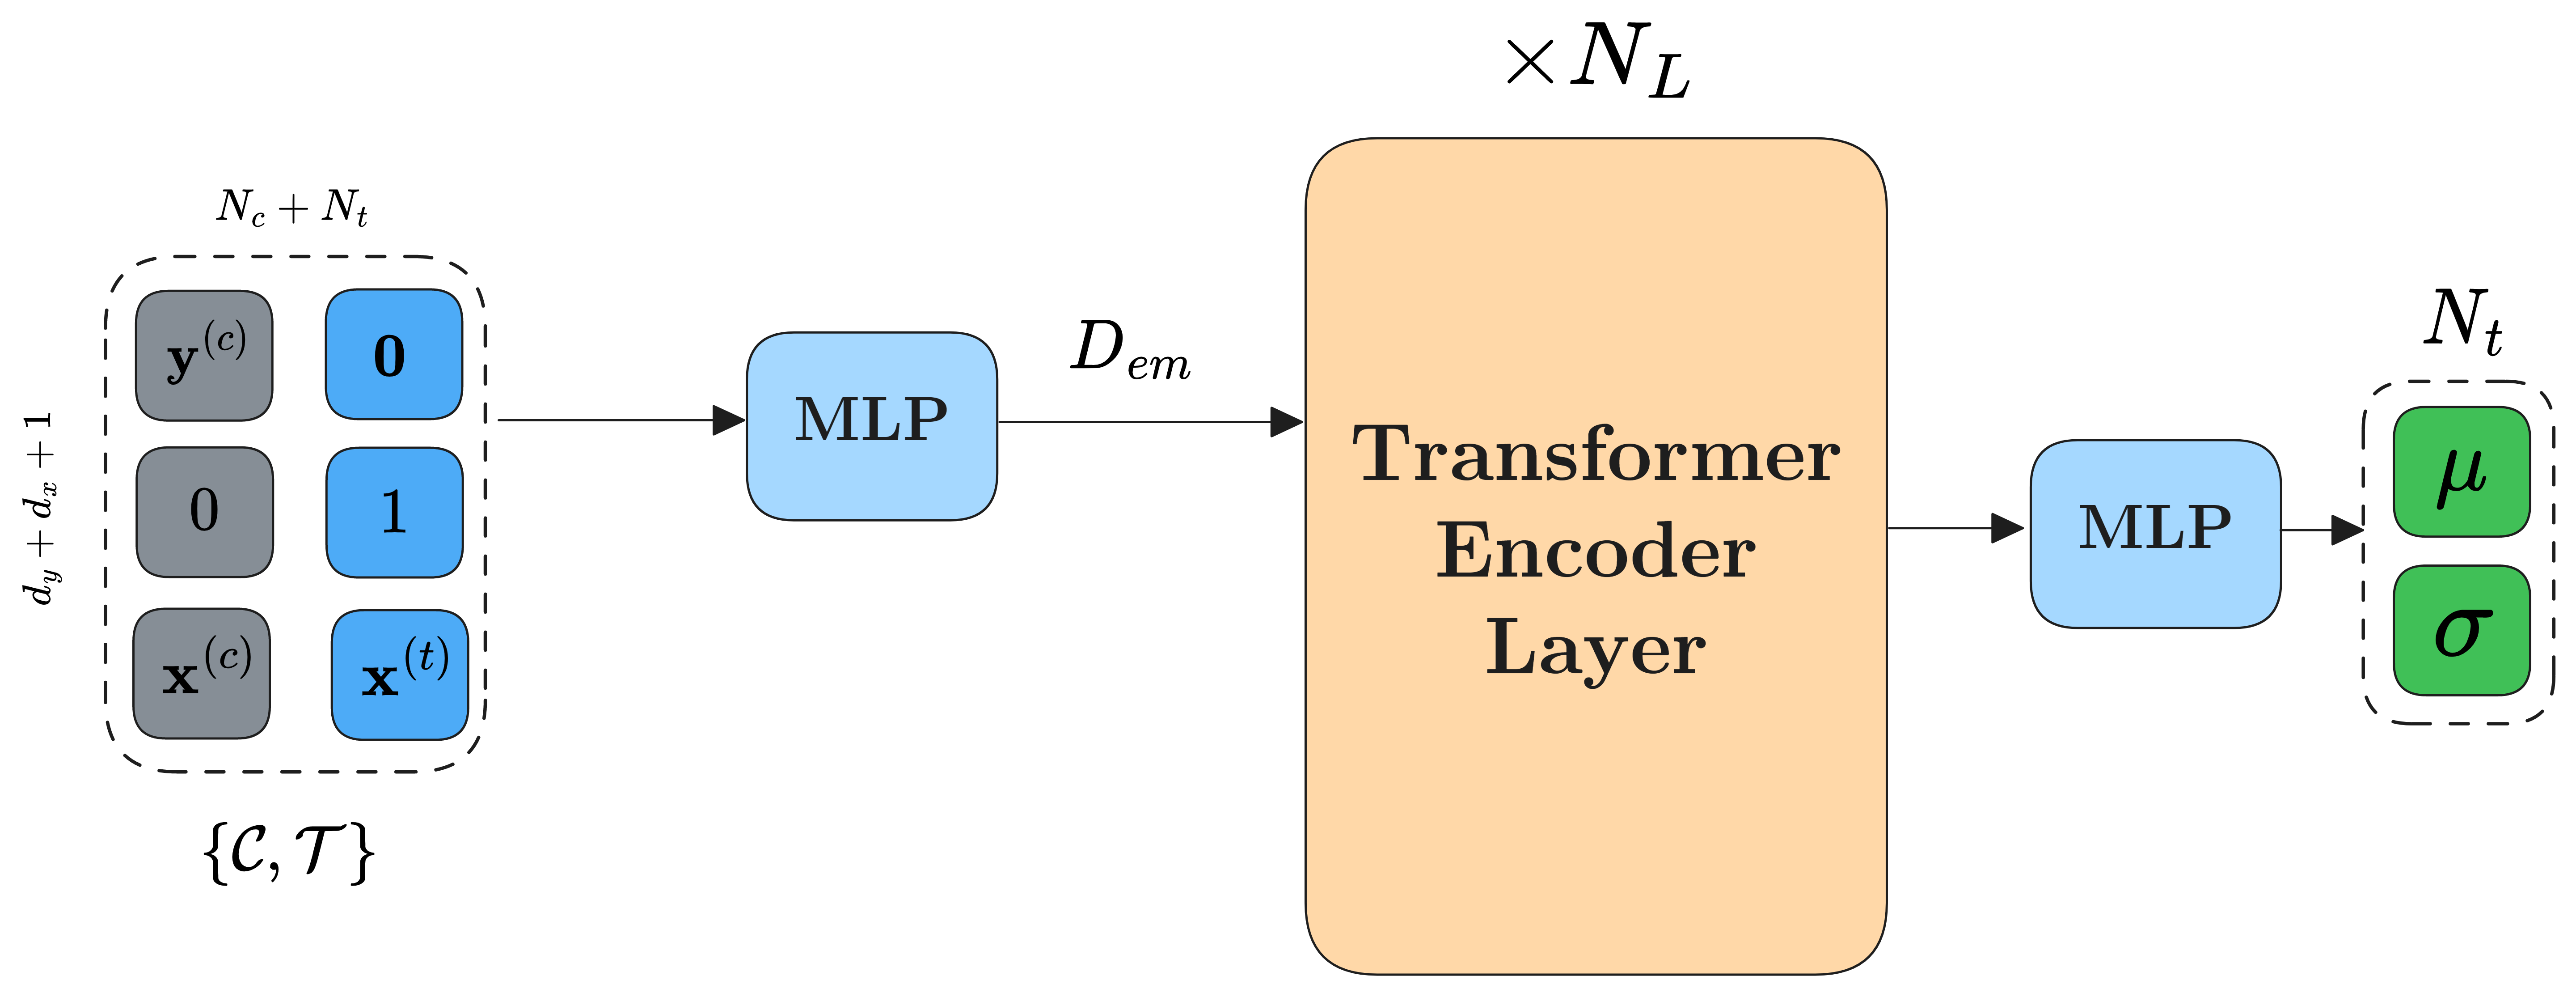
\includegraphics[width=0.9\textwidth]{./tnp.png}
	\caption{Vanilla Transformer Neural Process Architecture. All the context and target sets are tokenized and passed through the Transformer Layer. The output of the Transformer Layer is passed through an MLP to generate the mean and variance of the predictive distribution.}
	\label{fig:tnp}
\end{figure}

\subsection{Performance}

One of the key benefits of Transformers (and attention) is the ability to have a global view of the data, analogous to an `infinite receptive field' in Convolutional Neural Networks. This allows the model to learn very complicated relationships across many length scales in the data. However, this can be a double-edged sword as the model can overfit to the data within its training region and fail to generalize to unseen data. 

Translation Equivariance is a key property behind CNNs which allow them to generalize excellently to unseen data by learning features irrespective of their position in the data. Such feature learning is critical to modelling real world data where the positions of the data do not matter as much as the relative relationships between the data points, e.g. in image classification the position of the object in the image does not matter as much as the features of the object itself. Transformers lack this property, causing them to generate random predictions when the data is shifted out of context as shown in Figure \ref{fig:tnp-fail}.

% Figure ./tnp-fail.png

\begin{figure}[H]
	\centering
	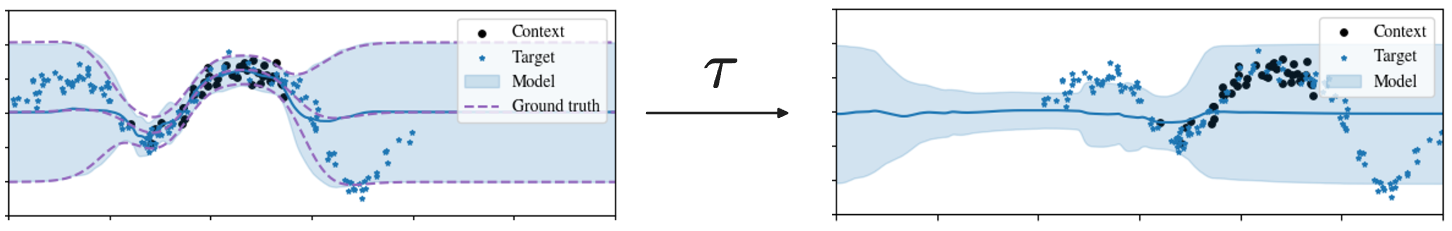
\includegraphics[width=0.9\textwidth]{./tnp-fail.png}
	\caption{Vanilla Transformer Neural Process failing to generalize in out of context data. The TNP successfully models the data in the context region (left) but fails to make predictions when the data is shifted (right).}
	\label{fig:tnp-fail}
\end{figure}

\emph{What if we could combine the best of both worlds?} Could we create a Translation Equivariant Transformer Neural Process (TETNP) which possesses the global view of the Transformer and the generalization properties of the CNN? This is the question we will investigate in the next section and is the main contribution of this work and \cite{anonymous2024translationequivariant}.



\section{Translation Equivariant TNP}
\label{sec:tetnp}

Recall, Translation Equivariance requires the model to yield the same output when the input is shifted. Such property must imply that the model only learns the relative distances between the data points ($\bm{x_i} - \bm{x_j}$) and \emph{not} the absolute positions of the data points. How could one enforce such a property in the Transformer Neural Process? The solution used is very simple, we add a term to the attention mechanisms in the Transformer to enforce the Translation Equivariance property!

Consider the standard attention mechanism in the Transformer, the attention weights are computed as:


\begin{align}
	\text{Attention}(\bm{Q}, \bm{K}, \bm{V}) &= \text{softmax}\left(\bm{E} \right) \bm{V}\\
	 \quad \bm{E_{ij}} &= \frac{\bm{q_i} \cdot \bm{k_j}}{\sqrt{d_k}}
\end{align}

To create a Translation Equivariant Attention mechanism we add a term to the attention weights which enforces the Translation Equivariance property. The new attention weights are computed with the following equation:

\begin{align}
	\label{eq:relative-attention}
	\text{Attention}(\bm{Q}, \bm{K}, \bm{V}, \bm{X}) &= \text{softmax}\left(\bm{E} + F(\bm{\Delta}) \right) \bm{V}\\
	\quad \bm{E_{ij}} &= \frac{\bm{q_i} \cdot \bm{k_j}}{\sqrt{d_k}}\\
	 \quad \bm{\Delta_{ij}} &= \bm{x_i} - \bm{x_j}
\end{align}

Where $F$ is some function that introduces non-linearity into the attention weights and is applied to each entry of the matrix independently ($F(\bm{\Delta})_{ij} = F(\bm{\Delta_{ij}})$), we will investigate the effect of different functions in the experiments later on. It is clear to see that if all the input locations are shifted by a constant $\bm{\tau}$, the relative term will remain the same $\bm{F(\Delta_{ij})} = F(\bm{x_i} + \bm{\tau} - \bm{x_j} - \bm{\tau}) = F(\bm{x_i} - \bm{x_j})$ and the attention weights will remain the same.

Importantly since we are enforcing the Transformer to learn the relative distances between the data points, we must remove the $\bm{x}$ values from the tokenization of the data points. The tokenization of the data points is now:

\[
	\bm{t_i} = \begin{cases}
		\text{MLP}(\texttt{cat}[0, \bm{y_i}]) & \text{if } i \leq N_c \\
		\text{MLP}(\texttt{cat}[1, \bm{ 0}]) & \text{if } i > N_c
	\end{cases}
\]


% Figure ./tetnp.png

\begin{figure}[H]
	\centering
	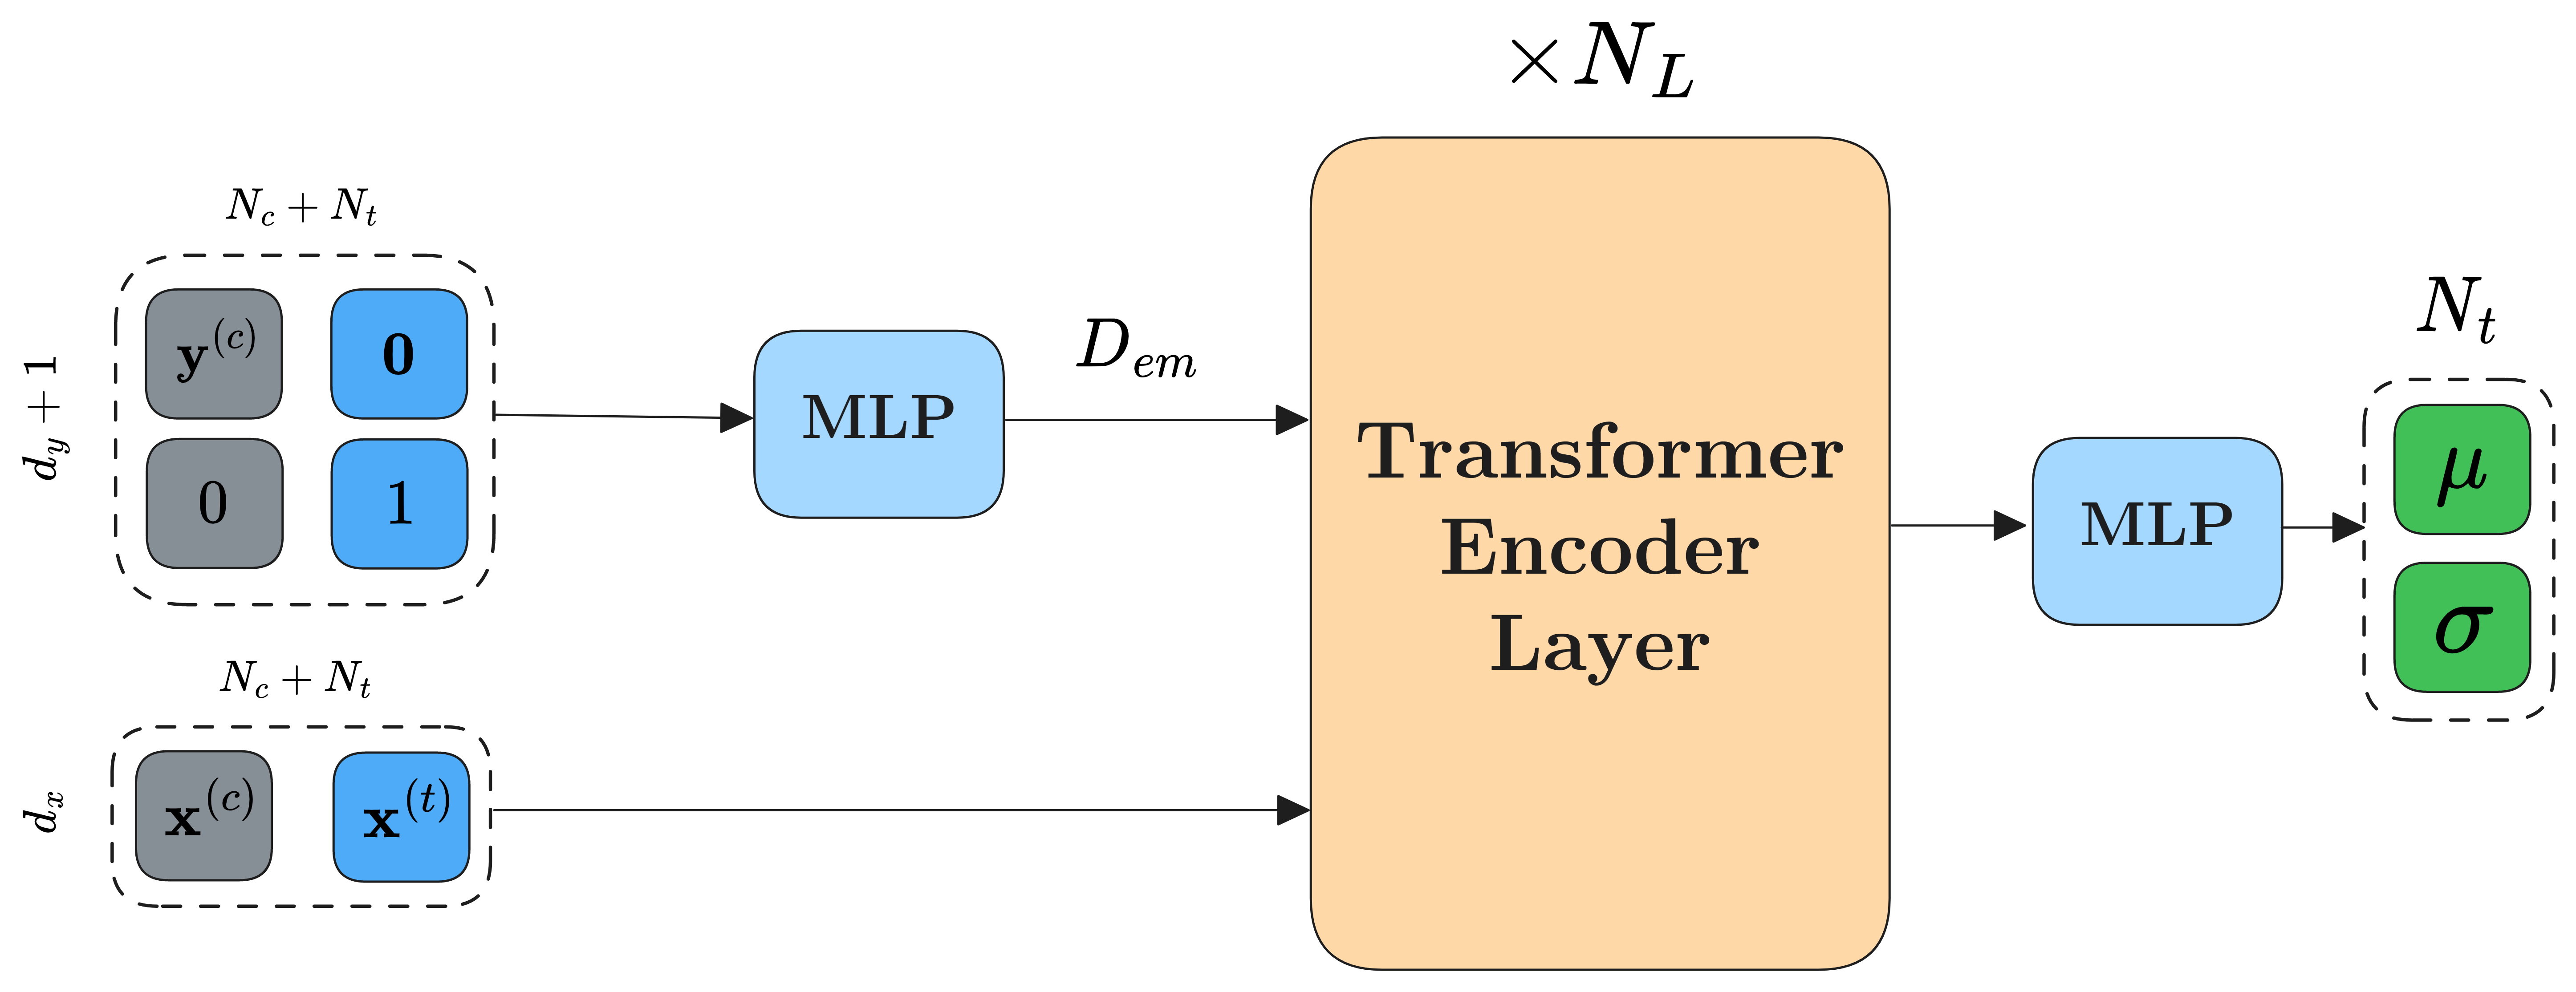
\includegraphics[width=0.9\textwidth]{./tetnp.png}
	\caption{Translation Equivariant Transformer Neural Process Architecture. All the outputs of the context and target sets are tokenized and passed through the Transformer Layer, whilst the input locations are passed in raw to the attention mechanism to enforce the Translation Equivariance property. The output of the Transformer Layer is passed through an MLP to generate the mean and variance of the predictive distribution.}
	\label{fig:tetnp}
\end{figure}


A benefit of removing the $\bm{x}$ values from the tokenization is that the tokens only need to encode the $\bm{y}$ values, reducing the dimensionality of the tokens whilst also separating the encoding for $\bm{x}$ and $\bm{y}$ values which could be beneficial for the model as in the vanilla TNP the model loses distinction between the $\bm{x}$ and $\bm{y}$ values since they are embedded together.







% As previously stated, the performance of the transformer can be tweaked by ajusting the hyperparameters of the model. 

% \subsection{Requirements}

% As NPs are a meta-learning method they should be trained on a context set which is a subset of a larger dataset. In this example, say we sample $N$ $x-y$ pairs from a process $\mathcal{F}$, we designate the first $N_c$ pairs as the context set and the remaining $N-N_c$ pairs as the target set, or mathematically $\mathcal{C} = \{(x_i, y_i)\}_{i=1}^{N_c}$ and $\mathcal{T} = \{(x_i, y_i)\}_{i=N_c+1}^{N}$. The objective function is the maximum likelihood estimation of the target set given the context set autoregressively, or mathematically on the target set.


% \begin{equation}
% 	\mathcal{L}(\theta) = \mathbb{E}_{(x, y) \sim \mathcal{F}} \left[ \log p(y_{N_c+1:N} | x_{N_c+1:N}, \mathcal{C}; \theta) \right]
% 	\end{equation}

% Where $\theta$ are the parameters of the model and $y_{N_c+1:N}$ and $x_{N_c+1:N}$ are the target set. Since we pass the target set through the model autoregressively, the objective function can be rewritten as:

% \begin{equation}
% 	\mathcal{L}(\theta) = \mathbb{E}_{(x, y) \sim \mathcal{F}} \left[ \sum_{i=N_c+1}^{N} \log p(y_i | x_i, \mathcal{C}, x_{N_c+1:i-1}, y_{N_c+1:i-1}; \theta) \right]
% \end{equation}

% Where each conditional is modeled as a Gaussian distribution with mean and variance predicted by the model. 

% There are two important properties of TNPs that we need to build upon:

% \begin{itemize}
% 	\item \textbf{Context Invariance}: If we permute the context set, the model should not change its predictions
% 	 \item \textbf{Target Equivariance} If we permute the target set, the model should not change its predictions, e.g. we shift the target set by one point to the left, and the model's predictions should also shift by one point to the left.
% \end{itemize}

% \subsection{Autoregressive Transformer Neural Processes (TNP-A)}

% We can not implement the traditional Transformer as the inclusion of the positional encoding breaks the context invariance property since the positional encoding is dependent on the position of the points, but we need to allow the model to learn the relationships between $x$ and $y$ \textbf{pairs}. To do this, \cite{nguyen2023transformer} concatenates the $x$ and $y$ pairs together into a single vector for the context set and target set. They then add auxiliary tokens from the target set but with $y=0$ such that the dataset looks like

% \[
% 	 {(x_1, y_1), . . . ,(x_N , y_N ),(x_{N_c+1}, 0), . . . ,(x_N , 0)}
% \]

% As we can see the $x$ values from the target set effectively appear twice, the auxiliary tokens are used to represent the target set and then the corresponding $y$ values are used to train the model since those tokens are not auxiliary. To make this work, we must employ a masking scheme to allow:

% \bul{
% 	\item Context tokens to attend to themselves
% 	\item Target tokens to attend to context and previous target tokens
% 	\item Auxillary tokens to attend to context and previous target tokens
% }

% This model is referred to as the Autoregressive Transformer Neural Process (TNP-A) in \cite{nguyen2023transformer}.

\ifSubfilesClassLoaded{%
    \printbibliography{}
}{} 


\end{document}